


\documentclass[ps,accumulate,economy,slideColor,nototal]{prosper}
% use option  pdf or ps+accumulate, depending of wheter you print or not


%\newif\ifweb\webtrue    %%%%%% htmlonly geht irgendwie nicht
\newif\ifsolution\solutionfalse
\newif\ifworking\workingfalse


%%% Local Variables: 
%%% mode: latex
%%% TeX-master: "main"
%%% End: 


\Logo(-1.0,-1){\includegraphics[width=0.4cm]{tflogo.ps}}




\usepackage{hyperref}

\usepackage{pstricks,pst-node,pst-text,pst-3d}
\usepackage{epic,eepic,epsfig}

\usepackage{listings}
%\lstset{language=}
\lstset{basicstyle=\tiny\ttfamily}
%\usepackage{lstpseudo}
%\lstset{language=pseudo}   % pseudo defines the keywords etc
%\lstset{labelstyle=\tiny}  %
%\lstset{basicstyle=\tiny}



%%%%%%%%%%%%%%%%%%%%%%%%%%%%%%%%%%%%%%%%%%%%%%%%%%%%%
%%%%%%%%%%% The color names are from dvipsnam.def   %
%%%%%%%%%%%%%%%%%%%%%%%%%%%%%%%%%%%%%%%%%%%%%%%%%%%%%

\usepackage{graphics,color}
\usepackage{graphicx}



\definecolor{sectionshadecolor}{cmyk}{0.9,0.83,1,0.70}
\definecolor{myheadcolor}{named}{MidnightBlue}
\definecolor{myred}{named}{BrickRed}
\definecolor{mygreen}{named}{PineGreen}
\definecolor{mygreen}{named}{OliveGreen}
\definecolor{myblue}{named}{Periwinkle}
\definecolor{myblue}{named}{NavyBlue}
\definecolor{myblue}{named}{BlueViolet}
\definecolor{mygray}{named}{Gray}
\definecolor{myyellow}{named}{Yellow}
\definecolor{myorange}{named}{YellowOrange}


\newcommand{\mygray}  [1]{\textcolor{mygray}{#1}}
\newcommand{\myblue}  [1]{\textcolor{myblue}{#1}}
\newcommand{\mygreen} [1]{{\textcolor{mygreen}{#1}}}
\newcommand{\myred}   [1]{\textcolor{myred}{#1}}
\newcommand{\myyellow}[1]{\textcolor{myyellow}{#1}}
\newcommand{\myorange}[1]{\textcolor{myorange}{#1}}

\newcommand{\unimportant}[1]{\textcolor{mygray}{#1}}
\newcommand{\important}  [1]{\textcolor{myblue}{#1}}
\newcommand{\importantx} [1]{\textcolor{mygreen}{#1}}
\newcommand{\importantxx}[1]{\textcolor{myred}{#1}}
%\newcommand{\sectionshade}[1]{\colorbox{sectionshadecolor}{#1}}
\newcommand{\sectionshade}[1]{\colorbox{myheadcolor}{#1}}

%%%% KAI
%\FontTitle{\usefont{T1}{phv}{b}{sl}\fontsize{14.4pt}{12pt}\selectfont\myred}{%
%   \usefont{T1}{phv}{b}{sl}\fontsize{14.4pt}{12pt}\selectfont\black}
%\FontText{\darkblue\usefont{T1}{phv}{m}{n}\fontsize{12pt}{11pt}\selectfont}{%
%   \black\usefont{T1}{phv}{m}{n}\fontsize{12pt}{11pt}\selectfont}


\FontTitle{\usefont{T1}{phv}{b}{sl}\fontsize{14.4pt}{12pt}\selectfont}{%
   \usefont{T1}{phv}{b}{sl}\fontsize{14.4pt}{12pt}\selectfont\black}
\FontText{\black\usefont{T1}{phv}{m}{n}\fontsize{12pt}{11pt}\selectfont}{%
   \black\usefont{T1}{phv}{m}{n}\fontsize{12pt}{11pt}\selectfont}


\newrgbcolor{LemonChiffon}{1. 0.98 0.8}
\newrgbcolor{LightBlue}{0.68 0.85 0.9}


\newenvironment{myslide}[1]   {\begin{slide}{#1}}{\end{slide}}


\usepackage{fancybox}  % Fancybox redefines. filedate

%%% Local Variables: 
%%% mode: latex
%%% TeX-master: "main"
%%% End: 

%\newcommand{\kommentar}[1]{[{\small\em #1}]

\newcommand{\Slime}{\textsc{Slime}}
\newcommand{\cvs}{cvs}
\newcommand{\Java}{\textsc{Java}}
\newcommand{\SMV}{\textsc{Smv}}
\newcommand{\Cplusplus}{C$^{++}$}
\newcommand{\javadoc}{\textsc{javadoc}}

\newcommand{\Int}    {\mathit{Int}}
\newcommand{\Bool}   {\mathit{Bool}}


\newcommand{\team}[1]{\textbf{Responsible:} #1\bigskip{}}



\newcommand{\bnfdef}{::=}
\newcommand{\bnfbar}{\ensuremath{\mid}}
\newcommand{\of}    {\ensuremath{\mathrel{:}}}
\newcommand{\without}{\backslash}
\newcommand{\ltrue}   {\mathit{true}}
\newcommand{\lfalse}  {\mathit{false}}

\newcommand{\suchthat}{\mathrel{\mid}}
\newcommand{\union}  {\cup}
\newcommand{\intersect}  {\cap}
\newcommand{\sizeof}[1]  {{\mid}{#1}{\mid}}
\newcommand{\sem}    [2]        {[\![#2]\!]_{#1}}      %semantics

\newenvironment{diagram}{\begin{displaymath}}{\end{displaymath}}

%\newcommand{\inputcode}[2][Code]   {
%  {\small
%  \mbox{}
%  \newline
%  \mbox{}
%  \hrulefill
%  \verbatiminput{#1/#2.java}
%  \hrulefill}}




\newcommand{\inputcode}[2][.]{
  {\footnotesize
  \mbox{}
  \newline\nopagebreak{}
  \mbox{}
  \hrulefill
  \lstinputlisting{#1/#2}
  \hrulefill}}

\newenvironment{code}{%
%  \small\mbox{}\nopagebreak{}\mbox\hrulefill{}
  {\begin{lstlisting}{}}}{%
  {\end{lstlisting}}}





%%%%%%%%%%%%%%%%%%%%%%%%%%%%%%%%%%%%%%% macros for semantics of SFC's

%%% RULES 


\newenvironment{ruleset}{
  \mbox{}\noindent\hrulefill\begin{displaymath}
    \renewcommand{\arraystretch}{1.6}\begin{array}[b]{l}}{
  \end{array}\end{displaymath}\hrulefill\mbox{}}




\newcommand{\treefont}{\small}
\newcommand{\leaf}[1]{{\begin{array}{c} #1 \end{array}}}
\newenvironment{proofleaf}{\begin{array}{c}}{\end{array}}

\newcommand{\namedruletree}[3]{{
     \treefont
     \prooftree 
       {\leaf{#2}}
     \justifies
       #3
     \using \rn{#1}
     \endprooftree
     }}                             

\newcommand{\ruletree}[2]{\namedruletree{}{#1}{#2}}


\newcommand{\rn}[1]{\mbox{\textsc{#1}}}   %% determines the font
\newcommand{\andalso}{\quad\quad}
\newcommand{\infrule}[3]{\namedruletree{#1}{#2}{#3}\andalso}
\newcommand{\scinfrule}[4]{\namedruletree{\mbox{$#4$}\quad\quad #1}{#2}{#3}\andalso}
\newcommand{\infax}[2]{
  \treefont
  #2\quad\quad \rn{#1}\andalso
  \andalso
  }
\newcommand{\scinfax}[3]{
  \treefont
  #2\quad \mbox{$#3$\quad\quad#1}
  \andalso
}




%%% SFCs
\newcommand{\init}          {\mathit{init}}
\newcommand{\act}           {\mathit{act}}
\newcommand{\Act}           {\mathit{Act}}
\newcommand{\States}        {\mathit{States}}
\newcommand{\Status}        {\mathit{Status}}
\newcommand{\Steps}         {\mathit{Steps}}
\newcommand{\Store}         {\mathit{Store}}
\newcommand{\Var}           {\mathit{Var}}
\newcommand{\Varin}         {\Var_{\mathit{in}}}
\newcommand{\Varout}        {\Var_{\mathit{out}}}
\newcommand{\Varloc}        {\Var_{\mathit{loc}}}

\newcommand{\src}           {\mathit{src}}
\newcommand{\target}        {\mathit{tar}}
\newcommand{\guard}         {\mathit{guard}}
\newcommand{\Expr}          {\mathit{Expr}}
\newcommand{\OF}            {\mathrel{:}}

\newcommand{\setto}[2]             {{\scriptstyle [#1\mathop{\mapsto}#2]}}  %setto{x}{v} : [x|->v]  {}
\newcommand{\substfor}[2]   {}

\newcommand{\inputstatus}       {\mathsf{I}}%{\mathit{WAITINPUT}}
\newcommand{\calcstatus}[1]     {\mathsf{C}(#1)}%{\mathit{DONEINPUT(#1)}}
\newcommand{\outputstatus}[1]   {\mathsf{O}(#1)}%{\mathit{FINISHED(#1)}}









%\newenvironment{diagram}{\begin{displaymath}}{\end{displaymath}}


\newcommand{\edge}[1]            {\longrightarrow_{#1}} %

%%% semantical steps
\newcommand{\trans}[1]             {\rightarrow_{#1}}
\newcommand{\transin}[1]           {\trans{?#1}}
\newcommand{\transout}[1]          {\trans{!#1}}








%%% Local Variables: 
%%% mode: latex
%%% TeX-master: t
%%% End: 

%\input{macros-local}



\title{Programming-in-the-many: 
  \\ \Slime\\ }
\subtitle{ \small Summer 2002}
\slideCaption{Slime, Summer 2002}
%\subtitle{subtitle}
\author{%
  \href{http://www.informatik.uni-kiel.de/~kst}{Karsten Stahl}
  \quad
  \href{http://www.informatik.uni-kiel.de/~ms}{Martin Steffen}
  }

%\email{email1 email2}

\institution{
  \begin{minipage}[t]{8.0cm}
    \begin{center}
      \small \unimportant{\textit{Institut.\  f{\"u}r Informatik u.\  Prakt.\ Mathematik}}
      \\
      \small \unimportant{\textit{Christian-Albrechts Universtit{\"a}t zu Kiel}}\\
    \end{center}
  \end{minipage}
  }



\def\linefactor{5}
\def\smalllinefactor{3}
\begin{document}
\DefaultTransition{Dissolve}
\maketitle{}

%----------------------------------------------------------------------

%%%%%%%%%%%%%%%%%%%%%%%%%%%%%%%%%%%%%%%%%%%%%%%%%%%%%%%%%%%%%%%%%%%%%%%%%%%%






\begin{myslide}{Slime}
  \begin{quote}
    \important{S}equentia\important{l} Funct\important{i}on Charts
    \important{M}odeling \important{E}nvironment
  \end{quote}
  \begin{itemize}
  \item \important{SFC}
    \begin{itemize}
    \item one of various  description languages for micro
      controllers
    \item international standard (IEC 61131)
    \item  Petri-net like semantics
    \item here: ``\important{poor man's SFCs}'': simplified, but with
      \important{formal} operational semantics
    \end{itemize}
  \end{itemize}
\end{myslide}

\begin{myslide}{Results}
  \begin{itemize}
  \item runnable tool, all modules integrated, executable under jdk-1.4
    \begin{itemize}
    \item graphical interface for editing
    \item checks (type checking, well-formed checking)
    \item parser
    \item simulator
    \end{itemize}
  \item \important{CD-Rom} with jar'ed tool (+ doc + sources + repos
    \ldots)
  \end{itemize}
\end{myslide}


\begin{myslide}{SFC example}
  

\vspace{-1cm}

  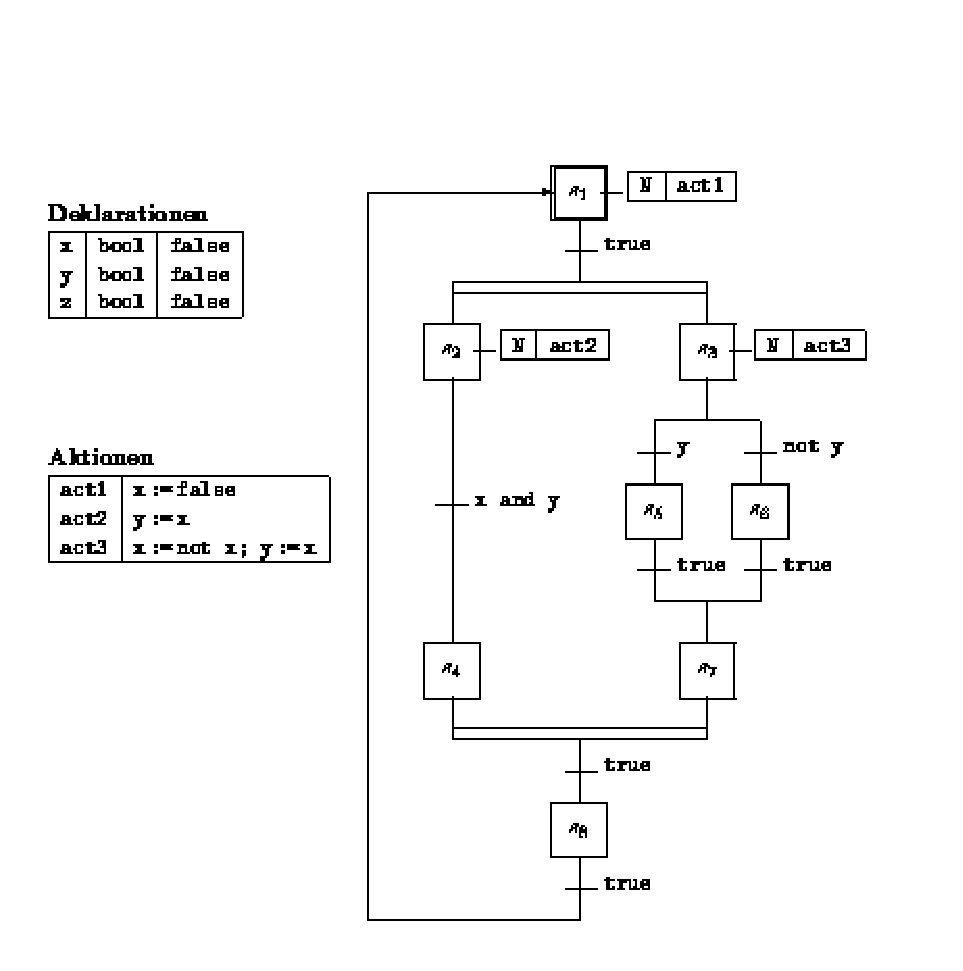
\includegraphics[height=7.5cm]{../requirements/sfc-figure}

\end{myslide}




\begin{myslide}{Develoment process}
  \begin{itemize}
  \item \important{CVS}, modules as packages
  \item Error-list, Status list
  \item email-list
  \item public \important{web-page} including \javadoc{} documentation
  \item weekly progress \important{report}
  \item 3 \important{review} meetings, including this one.
  \end{itemize}
\end{myslide}


\begin{myslide}{Timeline (planned and actual)}
  \begin{center}
   \includegraphics[height=6cm]{timeline.eps}  
    \end{center}
\end{myslide}



\begin{myslide}{Error reporting}
  \begin{lstlisting}{}
 --------------------------------------------------------
  Error <nr>:    <short description>
    package:     <in which package/class does it occur
    status:      reported|confirmed|non-confirmed|repaired
                 repaired-confirmed

               + <date> + <author>
   
    class:       fatal|non-fatal|
                 feature-request|coding convention violation ....

    description: <longer description, hints for repair>
   -----------------------------------------------------
  \end{lstlisting}
\end{myslide}



\begin{myslide}{Statistics}
  \begin{itemize}
  \item 13 official meetings
  \item 4 iterations of the requirement specification
  \item \important{> 500} emails concerning \Slime\ in my
    mailbox\footnote{including those exchanged directly with the
      participants, but without the more than 700 cvs-log emails.}
  \item approximately
    \begin{itemize}
    \item \important{100} officially reported errors\footnote{none
        confirmed \ldots}
    \item \important{170} Java files
    \item \important{200} class files, i.e. 200 public classes
    \item \important{50} \LaTeX-files (doc, web-pages, requirements)
    \item handfull of other files (Makefiles, Error lists etc.)
    \end{itemize}
  \end{itemize}
\end{myslide}





\begin{myslide}{Good}
  \begin{itemize}
  \item it's over
  \item we have a running tool ready
  \item nice result for so few people
  \item task distribution
  \item good \important{specification}: \important{formal} operational
    semantics
  \end{itemize}
  
\end{myslide}
\begin{myslide}{Neutral/beyond our control}
  \begin{itemize}
  \item not much people, 
  \item lot of (late) drop outs,\footnote{people at the beginning:
      \important{11} (except coaches), at the end: \important{4}} and
    lately announced
  \end{itemize}
\end{myslide}

\begin{myslide}{Less good}
  \begin{itemize}
  \item \important{Attracting} students
    \begin{itemize}
    \item another topic?
    \item stressing collaborative  work over programming in \Java?
    \end{itemize}
  \item \important{laaaate} first code delivery (26.\ June) /compilation,
    \important{laaate} integration (with all the consequences)
  \item we always had quite some breaches of \important{interfaces}, but:
    this year was the first time, I had to \important{discuss} why this is
    should be avoided without much discussion
  \item communication
  \item no test group, no Error ever \texttt{confirmed}
  \end{itemize}
\end{myslide}

\begin{myslide}{Next time}
  \begin{itemize}
  \item first \emph{Readme} or first \important{written plan}
    \important{required} to be \important{checked-in} in after 2 weeks
  \item stricter, enforced cvs-strategy?: \important{enforced
    compilability} for checking-in?
\item user \important{logging} (currently, I don't know how, the official
  university's server can do it, but there are other disadvantages of that
  solution)?
  \item stricter surveillance (e.g.\ for absynt), \important{watches}
  \item no \important{separation} between gui and editor? But an explicit
    \important{test} group.
  \item other means of communication? (\emph{news-group?}, cvs-logs?)
  \end{itemize}
\end{myslide}














%%%%%%%%%%%%%%%%%%%%%%%%%%%%%%%%%%%%%%%%%%%%%%%%%%%%%%%%%%%%%%%%%%%
%% $Id: content.tex,v 1.20 2002-07-19 12:43:37 swprakt Exp $
%%%%%%%%%%%%%%%%%%%%%%%%%%%%%%%%%%%%%%%%%%%%%%%%%%%%%%%%%%%%%%%%%%%
%%% Local Variables: 
%%% mode: latex
%%% TeX-master: "main"
%%% End: 

%\bibliographystyle{alpha}
%\bibliography{string,specification,modcheck,crossref}




%----------------------------------------------------------------------


\end{document}


%%% Local Variables: 
%%% mode: latex
%%% TeX-master: t
%%% End: 






%%% Local Variables: 
%%% mode: latex
%%% TeX-master: t
%%% End: 
